
\label{sec::3_ip}
Since this work aims at achieving autonomous navigation for humanoid robots in a 3D environment, it is helpful to work in an image domain, which represent depth information. The depth map extraction from stereo images, which is based on a weighted least squares disparity map \cite{min2014fast}, will, therefore, be explained in section \ref{sec::31_dm}, while the subsequent section \ref{sec::32_cc}, introduces the reader to the camera's calibration, without which the depth map extraction would not work in real setups.

\FloatBarrier
\section{Depth Map Extraction}
\label{sec::31_dm}
The depth map is generated from stereo camera images via stereo block matching \cite{hamzah2010sum}. Since this method works best for edge filtered images, one has to obtain edge filtered images $\bm{E}$ from grayscale images $\bm{G}$ via a convolution with the Sobel kernel $\bm{S}_x$ along the horizontal axis \cite{sobel2014an} (equation \ref{eq::31_sobel_conv}. 
\begin{align}
	\bm{E} = \bm{S}_x*\bm{G}
	\label{eq::31_sobel_conv}
\end{align}
The principle goal, for the inference of depth information from two images, is to find points in the right image that correspond to points in the left image. In figure \ref{fig::31_stereo_camera}, one can see that a point $\bm{X}$, which is seen by the left camera, could in principle lie anywhere on the epipolar line at $\bm{x}'$, as seen from the right camera, if there is no depth information available. 
\begin{figure}[h!]
	\centering
	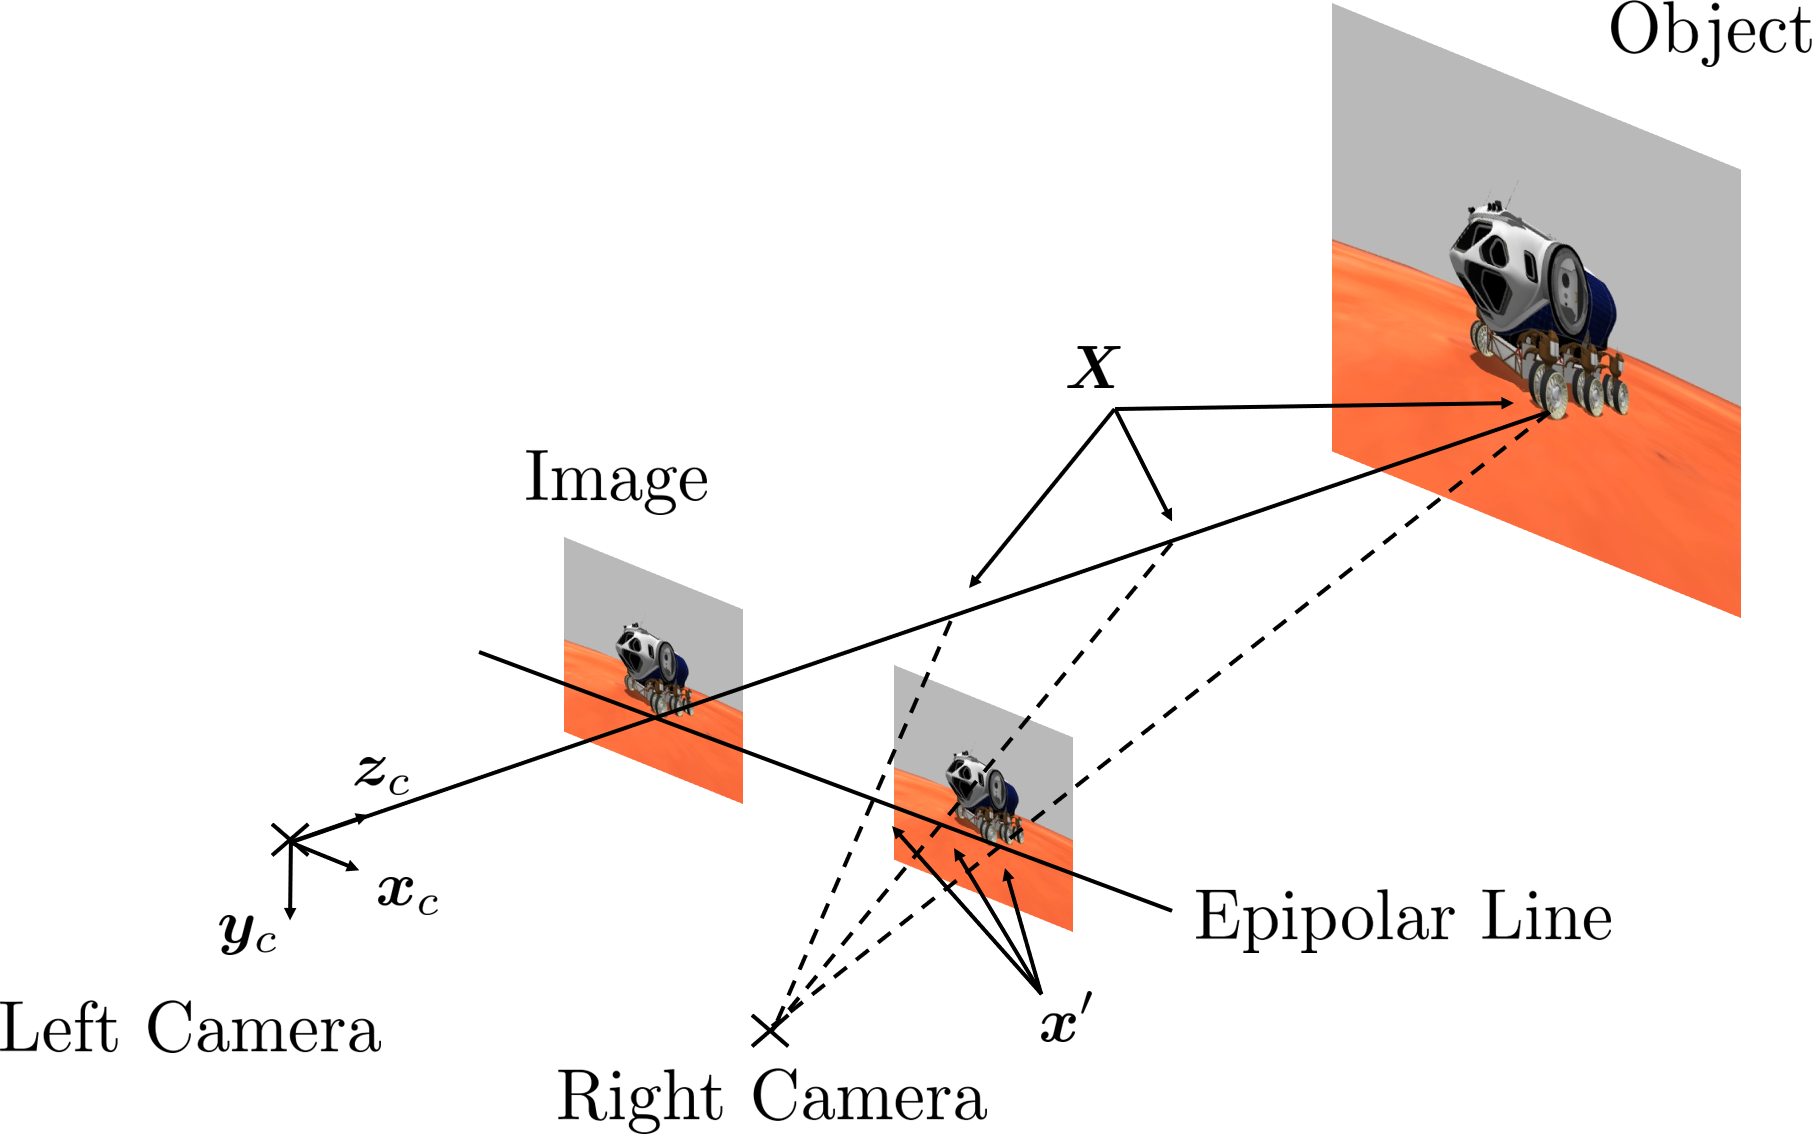
\includegraphics[scale=.28]{chapters/03_fundamentals_of_image_processing/img/stereo_camera.png}
	\caption{The stereo setup with a left and a right camera.}
	\label{fig::31_stereo_camera}
\end{figure}
It results that, to find correspondences, one only must search along the epipolar line, which is shown in figure \ref{fig::31_left_disparity_map}. Instead of looking for single-pixel correspondences, it is advised to search for whole block correspondences, since it reduces the noise drastically. Blocks of a defined block size $N$ are taken from the left image, and then the sum of absolute differences SAD is computed for every displacement $d$ in the right image, ranging from zero to number of disparities $D$ (equation \ref{eq::31_sad}, figure \ref{fig::31_left_disparity_map}).
\begin{align}
	\text{SAD}(d) = \sum_{x,y=0}^N |\bm{E}_\text{left}(x,y) - \bm{E}_\text{right}(x-d,y)|
	\label{eq::31_sad}
\end{align}
The disparity $d$ that minimizes the sum of absolute differences SAD is taken to serve as the best correspondence and is therefore used in the disparity map.
\begin{figure}[h!]
	\centering
	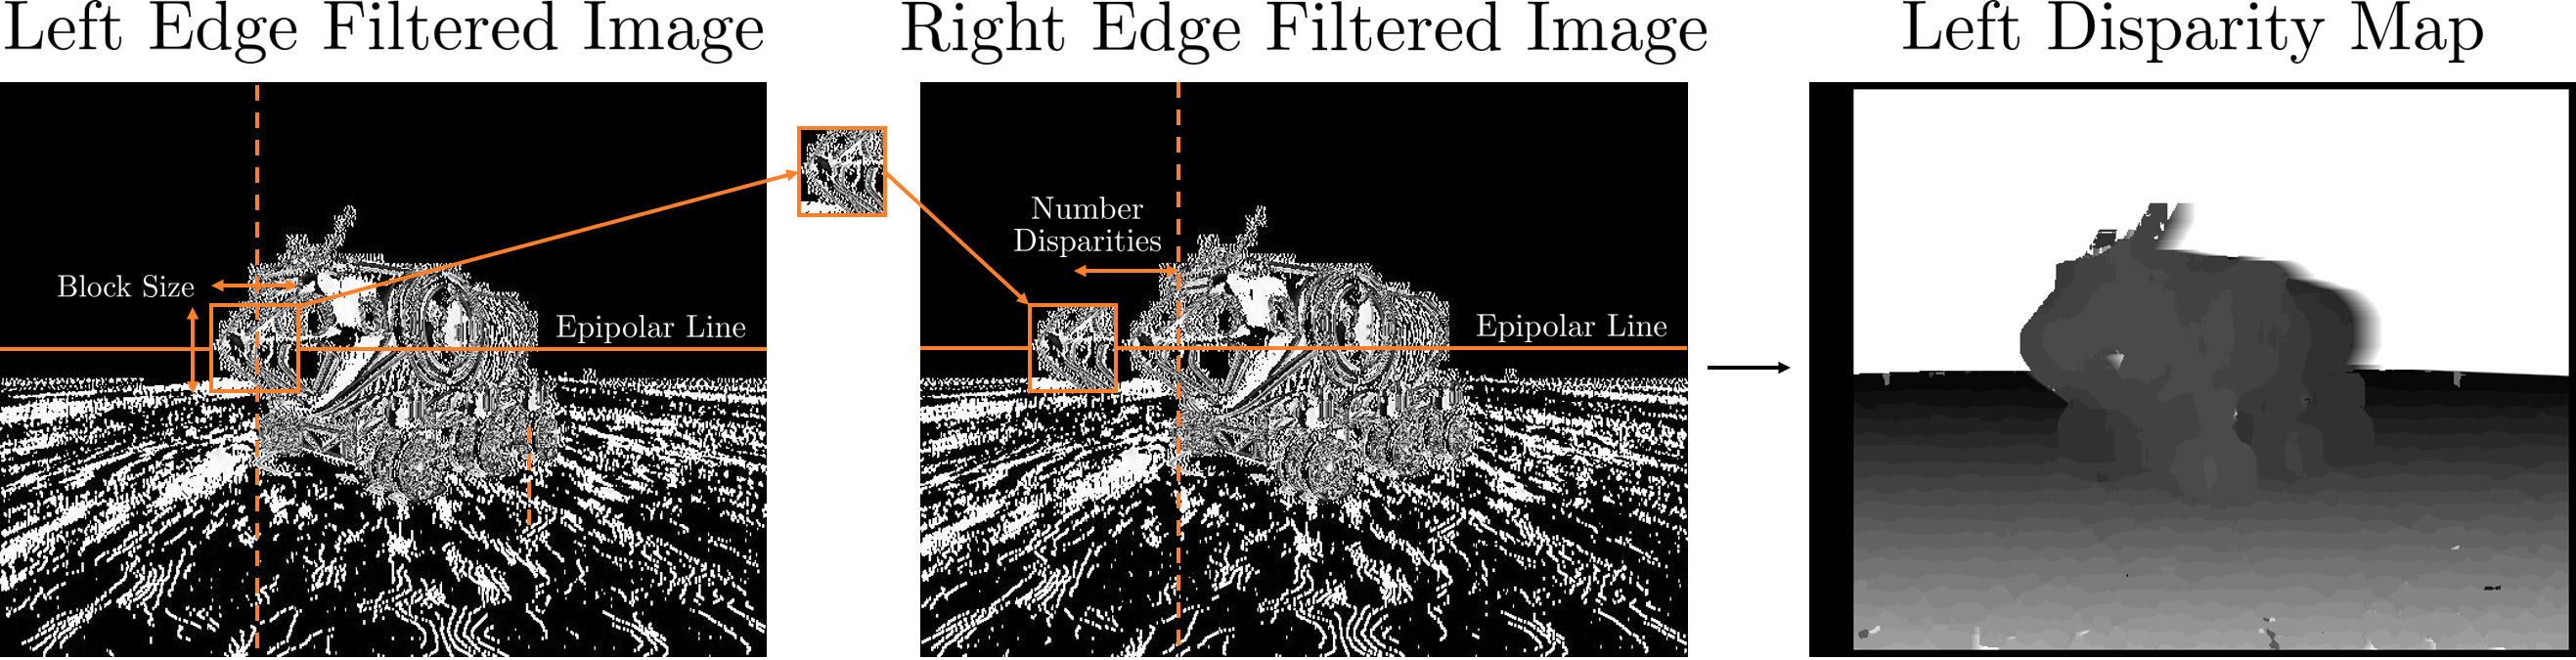
\includegraphics[scale=.28]{chapters/03_fundamentals_of_image_processing/img/left_disparity_map.png}
	\caption{Generation of the left disparity map by the block matching algorithm.}
	\label{fig::31_left_disparity_map}
\end{figure}
To further refine the disparity map, and especially to assure good results in textureless  regions, it is possible to apply a weighted least squares filtering, which is based on the confidence of depth measures. The confidence of depth measures is obtained from the variance $\text{Var}(\bm{D}) = \mathbb{E}\left[\bm{D}^2\right] - \mathbb{E}\left[\bm{D}\right]^2$ within the disparity map. Given the variance, one can compute the confidence map $\text{Con}(\bm{D})= \max\left(1-r\text{Var}(\bm{D}),0\right)$, which is a measures the certainty of the computed disparity, as follows
\begin{align}
	\text{Con}(\bm{D}) ,
\end{align}
where $r$ is a roll-off factor that defines the change of confidence with growing variance. The resulting disparity confidence map is used to outweigh outlying disparity values from the final weighted least squares disparity map. An additional measure for the prevention of accidentally assigned correspondences in the initial block matching algorithm is a left-right consistency check \cite{egnal2004stereo}. Therefore, the block matching algorithm is used in the right image, and it searches for correspondences in the left image. The left-right consistency $\bm{L}$ is then obtained by 
\begin{align}
	\bm{L}(x, y) = 
	\begin{cases}
	\min \left[\text{Con}(\bm{D}_\text{left})(x, y), \text{Con}(\bm{D}_\text{right})(x + d_\text{left}, y)\right] & \text{for } \Delta d < t  \\
	0 & \text{else}
	\end{cases},
\end{align}
where $d_\text{left}$ is the disparity of $\bm{D}_\text{left}$ at position $(x,y)$, $t$ is a threshold, and $\Delta d = \bm{D}_\text{left}(x, y) + \bm{D}_\text{right}(x + d_\text{left}, y)$. For the weighted least squares filtering, a consistency weighted disparity map $\bm{C}$ is computed via equation \ref{eq::31_cwd} (figure \ref{fig::31_weighted_least_squares_disparity}).
\begin{align}
	\bm{C}=\bm{L}\cdot\bm{D}_\text{left},
	\label{eq::31_cwd}
\end{align}
where $\cdot$ is an element-wise multiplication. The weighted least squares filter now results as the minimum of the energy function $J(\bm{U})$
\begin{align}
	J(\bm{U}) = \sum_{x,y}\left[(u_{x,y}-c_{x,y})^2+\lambda\sum_{(i,j)\in\mathcal{N}(x,y)}w_{x,y,i,j}(g)(u_{x,y}-u_{i,j})^2\right],
	\label{eq::31_energy_function}
\end{align}
where $c_{x,y}$ are single pixels of the consistency weighted disparity map, $\lambda$ is a smoothing parameter, and $w_{p,q}$ is a bilateral filter \cite{tomasi1998bilateral}, which takes the original grayscale image as guidance
\begin{align}
w_{x,y,i,j}(g) = exp(-|g_{x,y}-g_{i,j}|/\sigma),
\label{eq::31_weight}
\end{align}
with a range parameter $\sigma$. The final disparity map $\bm{D}_\text{final}$ is then obtained by normalizing the resulting image $\bm{U}$ with (figure \ref{fig::31_weighted_least_squares_disparity})
\begin{align}
	\bm{D}_\text{final} = \frac{\bm{U}}{\text{WLS}(\bm{L})},
	\label{eq::31_wls_final}
\end{align}
where $\text{WLS}(\bm{U})$ is the weighted least squares filtered version of the left-right consistency $\bm{L}$.
\begin{figure}[h!]
	\centering
	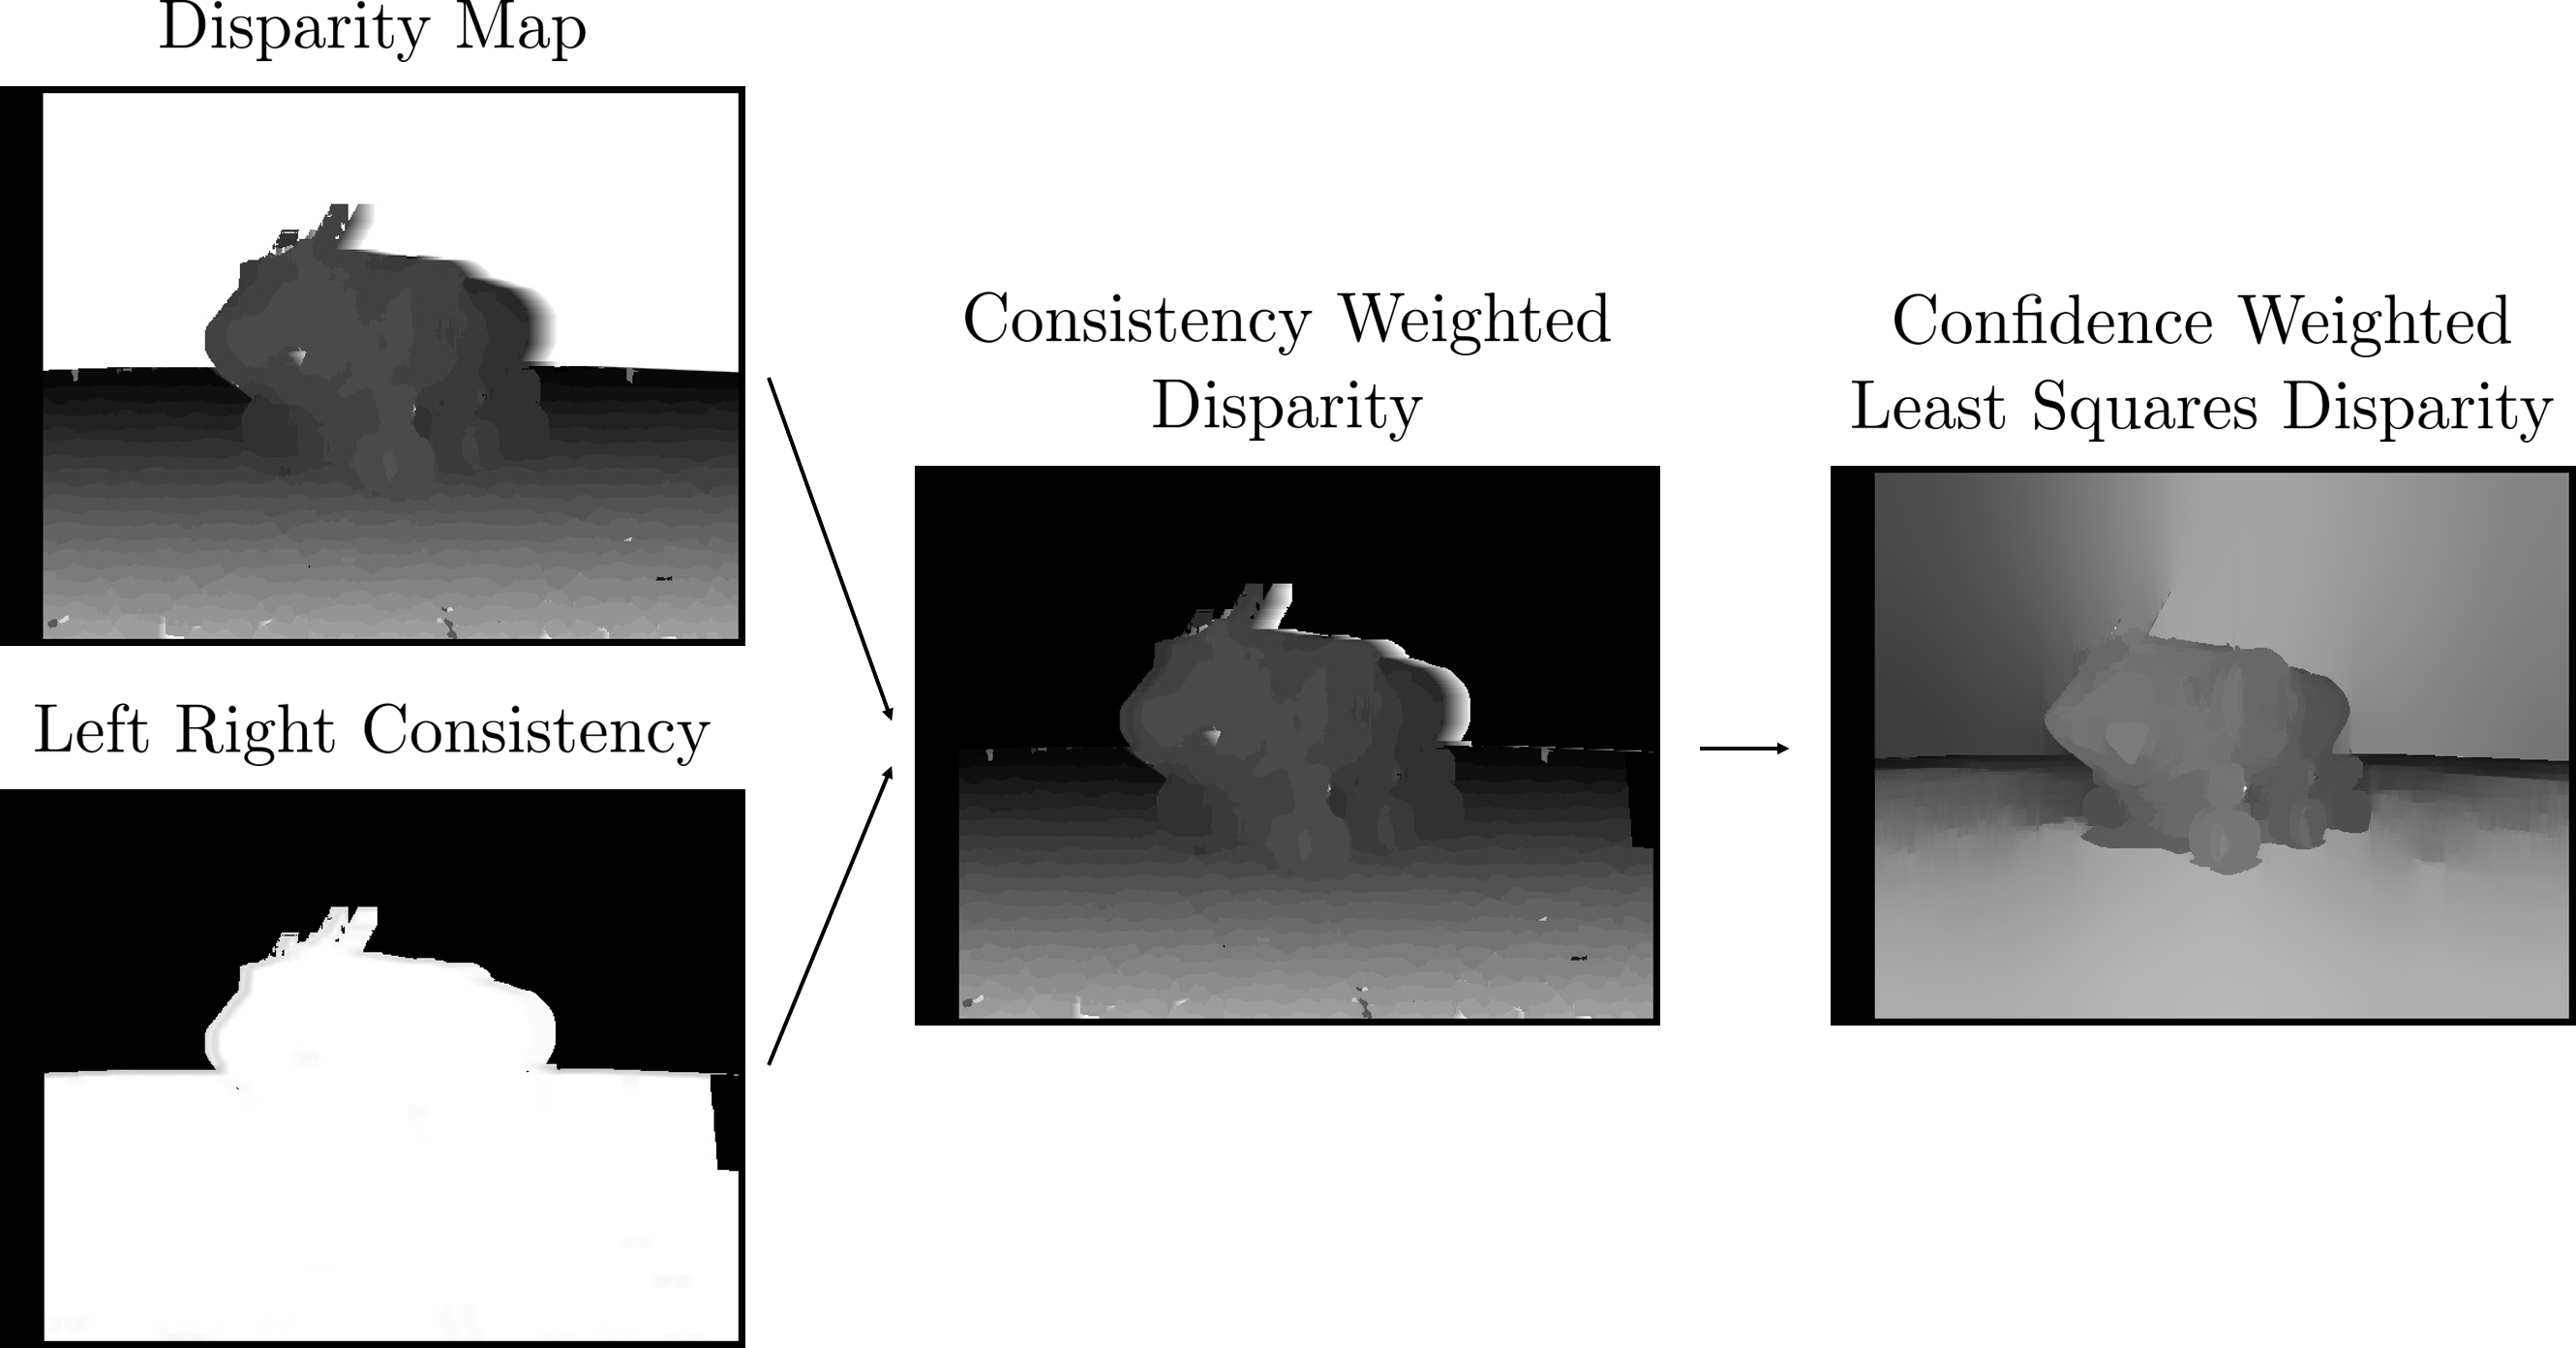
\includegraphics[scale=.28]{chapters/03_fundamentals_of_image_processing/img/weighted_least_squares_disparity.png}
	\caption{Generation of the confidence weighted least squares disparity from the disparity map, and the left-right consistency.}
	\label{fig::31_weighted_least_squares_disparity}
\end{figure}
Since the assumption of an only translated stereo camera pair is rarely correct, and there exist camera intrinsics that deform the observed image, it is required to calibrate the cameras for the algorithm to work properly, which is explained in the following section.

\FloatBarrier
\section{Mono and Stereo Camera Calibration}
\label{sec::32_cc}
A simple mathematical description for a camera is the pinhole model, which is shown in figure \ref{fig::32_pin_hole_camera}. The image plane therein lies behind the coordinate frame of the camera, but it is sufficient to describe the image in a virtual plane, which is located at a distance $f$ along the $z_c$-axis, where $f$ is the focal length.
\begin{figure}[h!]
	\centering
	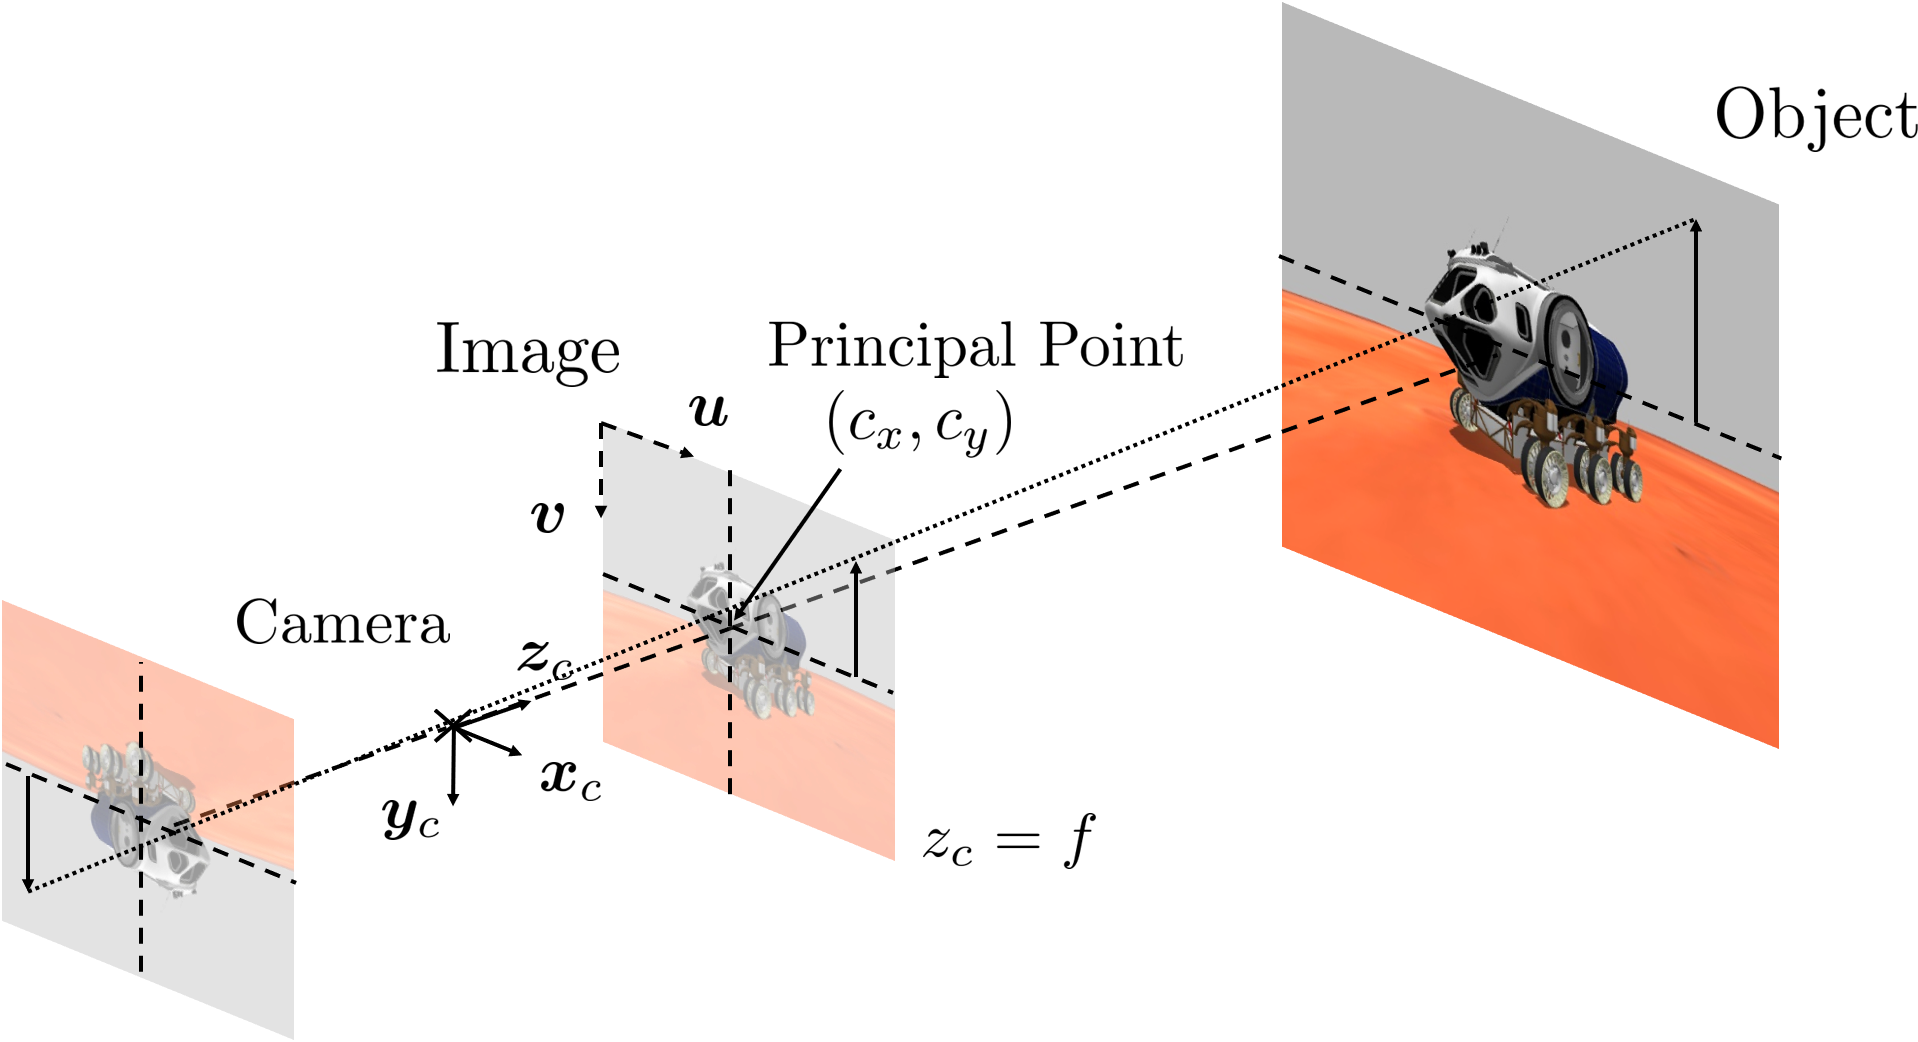
\includegraphics[scale=.28]{chapters/03_fundamentals_of_image_processing/img/pin_hole_camera.png}
	\caption{Pinhole camera model.}
	\label{fig::32_pin_hole_camera}
\end{figure}
A point $\bm{X}_c = (X,Y,Z)^T$ is then simply projected to the image plane by the camera matrix $\bm{K}$ with
\begin{align}
	\bm{x}_c = \bm{K}\bm{X}_c = \begin{pmatrix}
	f_x & 0   & c_x \\
	0   & f_y & c_y \\
	0   & 0   & 1
	\end{pmatrix}\bm{X}_c.
	\label{eq::32_focal_intrinsics}
\end{align}
Therein, $\bm{K}$ contains the intrinsic camera parameters, such as the focal lengths and the principal point. For a real setup, it is required to put a lens at the pinhole's position, adds radial and tangential distortion to the image, which can be modeled by \cite{duane1971close}
\begin{align}
	x_{c,u} &= x_{c,d}(1+k_1r^2+k_2r^4+k_3r^6) + p_1(r^2+2x_{c,d}^2) + 2p_2x_{c,d}y_{c,d} 
	\label{eq::32_x_dist}\\
	y_{c,u} &= x_{c,d}(1+k_1r^2+k_2r^4+k_3r^6) + 2p_1x_{c,d}y_{c,d} + p_2(r^2+2y_{c,d}^2),
	\label{eq::32_y_dist}
\end{align}
where
\begin{align}
	(x_{c,d}, y_{c,d}) = &\,\,\text{distorted image points within the camera frame $c$,} 
	\nonumber\\
		                 &\,\,\text{as projected onto the image plane}
	\nonumber\\ 
	(x_{c,u}, y_{c,u}) = &\,\,\text{undistorted image points within the camera frame $c$,}
	\nonumber\\
	                     &\,\,\text{as projected by an ideal pinhole camera}
	\nonumber\\
	k_n = &\,\,\text{n$^\text{th}$ radial distortion coefficient}
	\nonumber\\
	p_n = &\,\,\text{n$^\text{th}$ tangential distortion coefficient}
	\nonumber\\
	r = &\,\,\sqrt{x_{c,d}^2+y_{c,d}^2}.
	\nonumber
\end{align}
Together, the focal lengths, the principal point, and the distortion coefficients make up the unknowns within a camera model. Goal of the mono camera calibration is to find these coefficients from images of a well-known calibration pattern. Therefore, images of the calibration pattern are taken from different perspectives (figure \ref{fig::32_calibration_process}). 
\begin{figure}[h!]
	\centering
	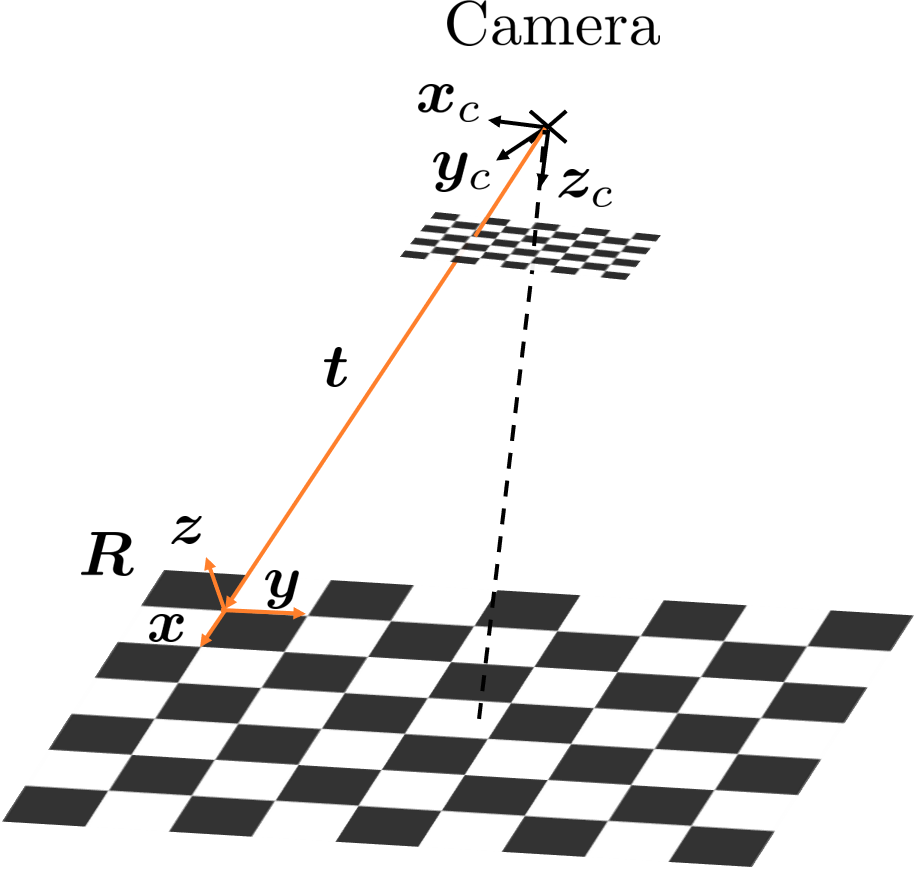
\includegraphics[scale=.28]{chapters/03_fundamentals_of_image_processing/img/calibration_process.png}
	\caption{Calibration pattern, as observed from the camera's coordinate system $C$. Within the object's coordinate system, all chessboard corners lie at a zero $z$-position.}
	\label{fig::32_calibration_process}
\end{figure}
The position of each corner can then be described by the square's size $a$ as follows
\begin{align}
	\bm{x}_{nm} = \begin{pmatrix}
	wa & ha & 0 & 1
	\end{pmatrix}^T,
	\label{eq::32_square_size}
\end{align}
which is expressed within homogeneous coordinates, and $w\in[0,W],h\in[0,H]$ are whole numbers, corresponding to the width and the height of the pattern. It is then required to find the rotation $\bm{R}$ and translation $\bm{t}$, which transforms the object points to the image plane. Therefore, a corner detecting algorithm finds the corners $\bm{x}_{c,wh}$ within the image plane. Under the assumption of known intrinsic camera parameters, $\bm{x}_{c,wh}$ are then being undistorted according to equations \ref{eq::32_x_dist} and \ref{eq::32_y_dist}. Each $\bm{x}_{nm}$ can then be transformed to the camera's frame, and further be projected onto the image plane via
\begin{align}
	\bm{x}_{c,wh} = \bm{K}\begin{pmatrix}
	\bm{R} & \bm{t}
	\end{pmatrix}\bm{x}_{wh},
\end{align}
where $\bm{R}$ describes the rotation, and $\bm{t}$ the translation of the camera frame to the object frame. Equations \ref{eq::32_x_dist} and \ref{eq::32_y_dist} then yield the undistorted image points $\bm{x}_{c,wh,u}$, which are reprojected by inverting the rotation and translation via
\begin{align}
	\bm{x}_{wh,u} = \begin{pmatrix}
	\bm{R} & \bm{t}
	\end{pmatrix}^{-1}\bm{x}_{c,wh,u},
	\label{eq::32_reprojection}
\end{align}
from which the re-projection error $\Delta x = ||\bm{x}_{wh,u} - \bm{x}_{wh}||_2$ is computed. The minimization of the re-projection error yields the intrinsic parameters \cite{zhang2000flexible}. Given the camera intrinsics of both cameras, it is possible to find the positions and orientations of both cameras with respect to the observed object. This allows to compute the fundamental matrix $\bm{F}$, which transforms points from the left camera's view $\bm{x}_{c_\text{left}}$, to points $\bm{x}_{c_\text{right}}$, as seen by the right camera via
\begin{align}
	\bm{x}_{c_\text{right}}^T\bm{F}\bm{x}_{c_\text{left}} = \bm{0}
\end{align}
The mapping enables us to rectify the left and the right image \cite{loop1999computing}, using the rectification transforms $\bm{R}_i$, which means that one can compute homography transforms that align epipolar lines within the images, which were previously defined by the fundamental matrix. These homography transforms map the images, as one observes them with the cameras, to a shared virtual plane, which is defined by the newly obtained projection matrices $\bm{P}_i$. Therefore, it enables one to apply the stereo block matching algorithm, which got introduced earlier, to the transformed images.